%!TEX root = ../template.tex
%%%%%%%%%%%%%%%%%%%%%%%%%%%%%%%%%%%%%%%%%%%%%%%%%%%%%%%%%%%%%%%%%%%%
%% chapter2.tex
%% NOVA thesis document file
%%
%% Chapter with the template manual
%%%%%%%%%%%%%%%%%%%%%%%%%%%%%%%%%%%%%%%%%%%%%%%%%%%%%%%%%%%%%%%%%%%%

\typeout{NT FILE demmon.tex}

\chapter{DeMMON}
\label{cha:demmon} 

DeMMon (Decentralized Management and Monitoring Overlay Network) is an overlay network aiming to create logical connections among nodes integrating the network, forming multiple tree-shaped networks. Then, it provides an API to request information about nodes and services running in the system, which is collected on-demand by the monitoring protocol via efficient information aggregation and dissemination using the tree structure.

In this chapter, we will begin by explaining the targeted environment and the operation of the overlay network, whose tree shape is the basis for the aggregation protocol. After, detail how the aggregation protocol performs aggregations in the tree, and lastly, list the operations exposed by the API and discuss how it interacts with the remaining components. \todo{insert refs to subsections ahead}

This solution, as observable in figure \ref{fig:demmon-overview}, is composed of three major components:

\begin{figure}[htbp]
    \centering
    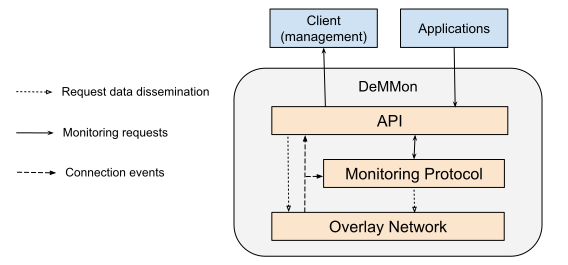
\includegraphics[width=\textwidth]{Chapters/Figures/DeMMon-arch-overview.pdf}
    \caption{An overview of the architecture of DeMMon}
    \label{fig:demmon-overview}
\end{figure}


\begin{enumerate}
    \item The overlay network, which strives to build a multi-tree-shaped network, nodes in this network use latency, node capacity, and a set of logical rules to change their location either from one tree to another or within their own tree.

    \item The monitoring protocol, which is a component that collects and disseminates information using the overlay network's established connections. It communicates via notifications and asynchronous request-replies with the overlay network to receive updates regarding established connections and connection failures. Lastly, it receives requests from the API to collect information.

    \item Lastly, the API receives updates from both the overlay network and the monitoring protocol, exposes the received information from those layers, and allows ingestion of new information. Furthermore, it allows issuing commands to collect new information, perform local aggregations periodically, or trigger issued alarms based on the respective conditions.
\end{enumerate}

\section{Overlay network} 
\label{sec:overlay_network}

\input{Chapters/membership/pseudocode/jlt-pseudocode.tex}

In this section, we discuss the design of the overlay network, which aims to build and maintain a latency and capacity-aware tree-shaped network (capacity represents one, or a combination of, values that denote the node's computing and networking power). We begin by providing the considered system model, then follow with an overview of the mechanisms responsible for building and maintaining the tree. Lastly, we conclude the chapter with a summary and discussion of the protocol.

\subsection{System Model}

The assumed system model is assumed to be a distributed scenario composed of nodes connected to the internet set-up such that they can send and receive messages via the internet (with an external IP or port-forwarding). We also assume that nodes are spread throughout a large area and have varied capacity values.

Regarding the fault model, we assume that all but a small portion of nodes (also known as the landmarks, which in our model represent DCs) can fail, and when other nodes fail, they do so in a crash-fault manner, stopping all emissions and receptions of messages. We assume landmarks have additional fault tolerance given their privileged infrastructure, and additionally, we assume other such as replication \cite{} mechanisms could be employed to ensure that faulty landmarks get replaced in case of failure. 
  
Finally, all nodes must run the same software stack with similar configuration settings and landmark values, installed a priori.

\subsection{Overview}

As previously mentioned, the main objective of the created protocol is to establish a latency and capacity-aware multi-tree-shaped network, rooted on the previously mentioned landmarks. Our motivations for choosing the tree structure for the network are the following: (1) to map the cloud-edge environment, by rooting the trees on nodes running DCs in the cloud, and creating a hierarchical structure for other, less powerful, nodes to be coordinated from the roots \todo{isto e esticar?} (2) to be able to map the heterogeneity of each device in the environment: by biasing the placement of nodes in the tree such that nodes with higher capacity are placed higher in the tree, and nodes with lower capacity are biased towards lower levels of the tree, nodes are used more or less according to their capacity values; (3) the tree structure can be easily employed to perform efficient aggregations, by propagating and merging values recursively from the lower to the higher levels of the tree, which is the basis for the aggregation protocol presented in \todo{add ref}; and finally, (4) by leveraging on the tree structure, nodes can propagate information efficiently, given that, in a network composed of N nodes, broadcasts require only N-1 message transmissions to reach all nodes in the network. 

The tree structure the protocol aims to establish and maintain can be observed in figure \todo{criar imagem para ilustrar estrutura resultante}, which, as previously referenced, is composed of multiple trees, and these are connected through their respective landmarks. The nodes connected to the landmarks, (denoted their \textbf{children}), may or may not form themselves be the parent of their own children. Intuitively, the \textbf{grandparent} of a certain node is their parents' parent, and the descendants of a certain node are constituted by all its children, and childrens' children, recursively. All nodes who share the same parent (\textbf{siblings}) are connected among themselves, forming a \textbf{group}, whose size is biased (but not guaranteed) to be within two configurable upper and lower bounds. Therefore, all nodes have active connections to their parent, children and siblings, this group of nodes denotes a node's \textbf{active view}. Nodes also have have knowledge of other nodes in the network, acquired via periodic semi-random periodic walks, which we will describe ahead. 

The devised algorithm is composed by three main mechanisms: (1) the \textbf{join} mechanism, which aims to establish the initial tree structures, (2) the \textbf{active view maintenance}, responsible for bounding the number of connections for each node, and optimizing the connections of each node, (3)  and finally \textbf{passive view maintenance}, responsible for collecting information about peers which are not in the active view, which are used for both fault tolerance and connection optimizations.

\subsubsection{Join mechanism}

The Join mechanism is the mechanism responsible for choosing the initial parent connection, which performs a greedy depth-first search to find a suitable low latency node in the network with more than zero children. This mechanism is the first to be executed by all nodes in the system, with the pseudocode presented in algorithm \ref{alg:memb:join}. 

% JOIN -----

\begin{algorithm}{}
\caption{Join Protocol} \label{alg:memb:join}
    % \setstretch{0.85}
\begin{algorithmic}[1]
    \asdtypes
        \State Node : <lat, parentIP, nrChildren, replied, IP, ID, coords, version, children<IP,  nrChildren\>\>
    \asdend
    \asdstate \label{alg:memb:join:state}
        \State contactedNodes \Comment{collection of all successfully contacted nodes}
        \State nodesToContact \Comment{nodes being contacted}
        \State landmarks \Comment{landmark nodes}
        \State joinTimeouts \Comment{collection of contacted nodes -> timerIDs}
        \State bestPeerLastLevel : Node \Comment{the best peer contacted so far in the join process}
        \State joinReqTimeoutTid \Comment{ timerID for join messages}
        \State self : Node \Comment{ myself}
    \asdend

\asdupon[Init(landmarks : IP[], selfIP, isLandmark)] \label{alg:memb:join:init}
    \State landmarks \asdassign landmarks 
    \State joinTimeouts, prevBestP \asdassign \{\}, nil
    \IfThenElse{isLandmark}
    {addLandmarkUntilSuccess(landmarks) \label{alg:memb:join:add_land}} 
    {contactNodes(landmarks) \label{alg:memb:join:contact_landm}} 
\asdend


\asdupon[receive(Join<>,sender)] \label{alg:memb:join:recv_join}
    \State sendMessageSideChannel(JoinReply<self.parent, self.node, self.children>, sender) 
\asdend
    
\asdupon[receive JoinReply(<parentIP, node, children>, sender) \&\& measuredLatency(lat)]  \label{alg:memb:join:recv_join_reply}
        \If{\asdin{node.IP}{nodesToContact}} 
            \If{\asdin{parentIP}{Landmarks}}
                \State self.coordinates[getIdx(landmarks, sender)] = lat
            \EndIf
            \State nodesToContact[node.IP].lat \asdassign lat
            \State nodesToContact[node.IP].children \asdassign children
            \State nodesToContact[node.IP].parent \asdassign parentIP
            \State nodesToContact[node.IP].replied \asdassign true
            \State cancelTimer(joinTimeouts[sender])
            \State delete(joinTimeouts, sender)
        \Else
            \State nodesToContact.delete(node)
        \EndIf
\asdend

\asdupon[(forall n $\in$ nodesToContact -> n.replied)] \label{alg:memb:join:cond_go}
    \State contactedNodes.appendAll(nodesToContact)
    \For{node in sortedByLatency(nodesToContact)}
        \If{(\asdnotin{node.IP}{landmarks}) \&\& node.nrChildren == 0} \label{alg:memb:join:verif_children}
            \State continue \Comment{check if node has enough children}
        \EndIf
        \If{prevBestP != nil \&\& (prevBestP.lat $\le$ node.lat || prevBestP.nrChildren < config.minGroupSize)} \label{alg:memb:join:verif_vs_prev}
            \State joinAsChild(prevBestP)
        \Else
            \State prevBestP \asdassign node \label{alg:memb:join:advance}
            \State toContact \asdassign [\asdin{c}{prevBestP.children} -> c.nrChildren > 0]
            \State contactNodes([c.IP for c in toContact])
        \EndIf
        \State return
    \EndFor
    \IfThenElse{prevBestP != nil} 
    {joinAsChild(prevBestP)}  
    {abortJoinAndRetryLater()} \label{alg:memb:join:join_base_case}
    \State return
\asdend

\asdupon[JoinTimeoutTimer(node) || NodeMeasuringFailed(node)] \label{alg:memb:join:exclusions}
    \IfThenElse{(L in Landmarks)}{abortJoinAndRetryLater()}{delete(nodesToContact[L])} 
\asdend

\asdupon[JoinRequestTimer(p : Node)]
    \If {sender == prevBestP}
        \If{p.parentIP != nil}
            \State prevBestP \asdassign contactedNodes[p.parentIP]
            \State joinAsChild(prevBestP)
        \Else
            \State abortJoinAndRetryLater()
        \EndIf
    \EndIf
\asdend

\asdupon[receive(JoinRequest<>, sender)]
    \State childID \asdassign addChildren(sender) \Comment{new chilren is established, and an ID is generated for it}
    \State sendMessageSideChannel(JoinRequestReply<childID, self>, p.IP)
\asdend
    
\asdupon[receive(JoinRequestReply<myID, parent>, sender)]
    \If {sender == prevBestP} 
        \State parent \asdassign sender \Comment{Adds Parent is established, join complete}
        \State cancelTimer(joinReqTimeoutTid)
        \State self.ID \asdassign parent.ID + "/" + myID \Comment{Later used in shuffle mechanism}
    \EndIf
\asdend

\asdprocedure[joinAsChild(p : Node)]
    \State joinReqTimeoutTid \asdassign setupTimer(JoinRequestTimer<p>, config.JoinTimeout)
    \State sendMessageSideChannel(JoinRequest<>, p.IP)
\asdend

\asdprocedure[contactNodes(ips : IP[])]
    \State nodesToContact \asdassign \{\}
    \State toContact \asdassign [Node<0,nil,0,false,lIP,false,[]> for ip in ips]
    \For{n in toContact}
        \State nodesToContact[n] \asdassign n
        \State MeasureNode(n) 
        \State sendMessageSideChannel(JoinMessage<>, n)
        \State joinTimeouts[n] \asdassign \asdassign setupTimer(JoinTimeoutTimer(n), config.JoinTimeout)
    \EndFor
\asdend

\end{algorithmic}
\end{algorithm}


Its first step (line \ref{alg:memb:join:state}) is to initialize the state of the joining node, composed by: (1) a map of type Node containing all successfully contacted nodes so far the join process, (2) a collection of type Node and a set of timer ids for each contacted node, (4) the best node contacted so far in the join process, (5) a timer id for contacting the chosen node in the join process, and finally (5) a variable of type Node denoting the peer itself. The type ``Node'' is a collection of attributes regarding a node, composed of latency measured, its current parent, number of children, whether the node replied to the message, its IP, and an array of its childrens' IP and children number.

Then, each node joins the system, the procedures taken to join the tree differ consonant the node is a landmark or not. Given that landmarks are the roots of the trees, they have no parent in the resulting overlay, and consequently, in the join algorithm, these nodes attempt to repeatedly establish a connection with other landmarks by sending a special message. Landmarks that receive this message will send a reply and establish a connection back (line \ref{alg:memb:join:add_land}), a joining landmark node only stops sending messages to other landmarks when the respective reply is received.

Nodes that are not landmarks begin the process of choosing their initial parent, initiated by sending a JOIN message via a temporary TCP channel, measuring the latency, and issuing ``joinTimers'' for all tree roots (line \ref{alg:memb:join:contact_landm}), then the node awaits the responses from the contacted nodes, during this process, the joining node listens for any ``joinTimers'' which have triggered, or until any of the node measurements has been unsuccessful (meaning contacted nodes have exceeded their reply timeout), if this happens, in the case of the contacted node being a landmark, the joining node aborts the join process and waits a configurable amount of time until attempting to re-join the overlay again. If the timed-out node is not a landmark, then that node is excluded from the remaining of the join process, and the join process is resumed as normal (line \ref{alg:memb:join:exclusions}).

When a node receives a JOIN message, it sends a JOINREPLY message back to the original sender containing: its parent, itself, and its children (line \ref{alg:memb:join:recv_join}). When the joining node receives the joinReply, it checks to see if it is not from a timed out node, or if the node's parent is not the same anymore, if any of these conditions are observed, then the reply is discarded. 

Then, whenever the joining node has either: received the JOINREPLY messages from all the contacted nodes, and stored the information (line \ref{alg:memb:join:recv_join_reply}), or they have been timed-out via the ``joinTimers'', it evaluates all contacted nodes, attempting to find the contacted node with the lowest latency which is a suitable parent by performing the following verifications:

\begin{enumerate}
    \item Verify if the node already has any children or if the node is a landmark (and can become parent of the joining node) (line \ref{alg:memb:join:verif_children}).
    
    \item Verify if there was a node already contacted which was a suitable parent and had lower latency, if there was, the joining node sends a JOINREQUEST and sets up a ``JoinRequestTimer'' for that node, and stops the verification process. (line \ref{alg:memb:join:verif_vs_prev})

    \item Verify if the current node has both enough children, and has the lowest latency up to this point in the join process, then the joining node assigns it as its best node so far and starts a new recursive step by sending JOIN messages and measuring the children of that node which themselves have more than one children (line \ref{alg:memb:join:advance}). Note that if none the current nodes' children are suitable parents (i.e. have no children themselves), then the condition in line \ref{alg:memb:join:cond_go} is triggered and the joining node will request the current best node to be its parent.
\end{enumerate}

If none of the verified peers was suitable to start a new recursive step (line \ref{alg:memb:join:join_base_case}) (either had no children or all verified nodes had higher latency than a previously contacted node), then the node joining node sends a ``JoinRequest'' to that node and sets up a ``JoinRequestTimer'' for the best previously contacted node (any node which receives a ``JoinRequest'' message replies with a ``JoinRequestReply''). 

The join process is concluded with both the reception of a ``JoinRequestReply'' and the establishment of the connection between the sender and receiver of the message. If the ``JoinRequestTimer'' timer triggers while waiting for the response, the node will recursively fall back to the parent of the selected node or re-join the overlay later in case there is no parent available. 

\subsubsection{Active view maintenance}

The second mechanism of the devised membership algorithm, called active view maintenance, is the mechanism responsible for maintaining the size of the groups. It achieves this by choosing new parents to form new groups using latency and node capacity as heuristics for the choice. This mechanism is coordinated by each parent, and is only done when the group exceeds its size limit. The information necessary to feed this mechanism is transmitted periodically from each children to their parents. 

The pseudocode for this mechanism is presentend in algorithm \ref{alg:memb:active_view_maint}, and starts by defining the necessary state: the nodes' active view (parent, children, and siblings), and an auxiliary map of sets, which holds the latencies of each children to every other children. (lines \ref{alg:memb:active_view_maint:state_start}-\ref{alg:memb:active_view_maint:state_end}). 

The mechanism starts with the propagation of information from the parent to the children and vice-versa. As observable in lines \ref{alg:memb:active_view_maint:update}-\ref{alg:memb:active_view_maint:update_end}), each parent transmits to its children a list of its current siblings, and propagates to its parent the latency to each of its siblings. Then, when this information is received (lines \ref{alg:memb:active_view_maint:update_recv_par} and \ref{alg:memb:active_view_maint:update_recv_chi}), it is merged into their local states for later use.

The second part of this mechanism is also periodic and is responsible for maintaining the group sizes by creating new groups, or sending children to already created groups (line \ref{alg:memb:active_view_maint:update_eval}) when necessary, this mechanism is only executed if the number of children exceeds the configured maximum number of children per parent (in order to keep group sizes close to full). Each node starts by merging all of its received latency pairs into a single set, where the node with the highest capacity is the first node of each pair (lines \ref{alg:memb:active_view_maint:update_eval_merge_start}-\ref{alg:memb:active_view_maint:update_eval_merge_finish}). Then, it iterates the added edges set by ascending order of latency, making the following steps:

\begin{enumerate}
    \item If the number of current children minus the nodes already sent to a lower level is lower than the middle point between the maximum size of a group, then the node concludes the mechanism (line \ref{alg:memb:active_view_maint:check_done_1})
    
    \item if the latency of the node pair that is being observed is higher than the parents latency to it, meaning it raises the overall latency of the system, and the current node size is lower than the configured maximum, then the process is concluded. (line \ref{alg:memb:active_view_maint:check_done_2})
    
    \item If any of the nodes was already sent to lower levels of the tree, then the current edge is skipped (line \ref{alg:memb:active_view_maint:check_done_3})
    
    \item Then, if the node wigh higher capacity of the edge pair has no children yet, the lower capacity node is added to its ``possibleChildren'' set, when this set has the same size of the minimum configured group size (i.e. the hifgher capacity node has enough candidates to form a new group), then the 
\end{enumerate}


\begin{algorithm}
    \caption{Membership protocol (Active view Optimization)} \label{alg:memb:active_view_maint}
    % \setstretch{0.85}
    \begin{algorithmic}[1]
        \asdstate
            \State parent \Comment{defined in join} \label{alg:memb:active_view_maint:state_start}
            \State children \Comment{defined in join} 
            \State siblings  
            \State childrenLatencies : dict<string:dict<string:number>> \label{alg:memb:active_view_maint:state_end} \Comment{Holds the latencies of each children to every other children}
        \asdend

        \asdrepeateveryx{config.updatePeriodicity} \label{alg:memb:active_view_maint:update}
            \If{parent != nil}
                \State sLatencies \asdassign set()
                \For{sibling in siblings}
                    \State sLatencies.append(<sibling.IP,sibling.measuredLatency)
                \EndFor
                \State sendMessage(UpdateChildStatus<children, siblingLatencies>, parent)
            \EndIf
            \For{child in chidren}
                \State sendMessage(UpdateParentStatus<self, chidren \\ child>)
            \EndFor
        \asdend \label{alg:memb:active_view_maint:update_end}

        \asdupon[receive(UpdateParentStatus<parent, children>, sender)] 
        \label{alg:memb:active_view_maint:update_recv_par}
            \If{sender == parent.IP}
                \State parent \asdassign parent
                \State self.ID \asdassign parent.ID + myID
                \State grandParent \asdassign grandParent
                \State siblings \asdassign siblings
            \EndIf
        \asdend

        \asdupon[receive(UpdateChildStatus<child, childSiblingLatencies>, sender)]\label{alg:memb:active_view_maint:update_recv_chi}
            \If{children[sender] != nil}
                \State children[sender]\asdassign child
                \State childrenLatencies[sender] \asdassign childSiblingLatencies
            \EndIf
        \asdend

        \asdrepeateveryx{config.evalGroupSize} \label{alg:memb:active_view_maint:update_eval}
            \If{len(children) <= config.maxGroupSize}
                \State return
            \EndIf
            \State childrenLatValues \asdassign set()
            \For{c1 in children} \label{alg:memb:active_view_maint:update_eval_merge_start}
                \For{<c2, lat> in childrenLatencies[c]}
                    \If{lat - c1.measuredLatency > d.config.maxLatDowngrade}
                        \State continue
                    \EndIf
                    \State isDowngrade \asdassign lat > c1.measuredLatency
                    \IfThenElse{c1.cap > c2.cap}
                    {childrenLatValues.add(<c1,c2,lat,isDowngrade>)}
                    {childrenLatValues.add(<c2,c1,lat,isDowngrade>)}
                \EndFor
            \EndFor \label{alg:memb:active_view_maint:update_eval_merge_finish}
            \State kickedNodes, newParents \asdassign set(),set()
            \State pChildren \asdassign dict<string,set<Node{>}{>} \Comment{set of potential children for each children}
            \State sortByLatency(childrenLatValues)
            \State idealGroupSize \asdassign config.maxSize - config.MinGroupSize
            \For{<c1,c2,lat,isDowngrade> in childrenLatValues}
                \If{len(children) - len(kickedNodes) <= idealGroupSize} \label{alg:memb:active_view_maint:check_done_1}
                    \State break
                \EndIf
                \If{len(children) - len(kickedNodes) <= config.maxSize \&\& isDowngrade} \label{alg:memb:active_view_maint:check_done_2}
                    \State break
                \EndIf
                \If{\asdin{c1}{kickedNodes} || \asdin{c2}{kickedNodes} ||  \asdin{lowerCapC}{newParents}} \label{alg:memb:active_view_maint:check_done_3}
                    \State continue
                \EndIf
                \If{c1.nrChildren == 0 \&\& newParents[c1] == nil}
                    \State pChildren[c1].append(c2)
                    \If{len(pChildren) >= config.MinGroupSize}
                        \If{len(children) - len(kickedNodes) - len(pChildren) > idealGroupSize || len(pChildren) >= config.maxSize}
                            \For{potentialChild in pChildren[c1]}
                                \State newParents <- newParents + c1
                                \State send(OptimizationPropose<c1>, potentialChild)
                                \State c1.nrChildren++
                                \State kickedNodes <- kickedNodes + potentialChild
                            \EndFor
                            \For{<nIP,pontentialChildrenTmp> in pChildren}
                                \State pontentialChildrenTmp.deleteAll(pChildren[c1])
                            \EndFor
                            \State pChildren[c1] \asdassign set<Node>
                            \State continue
                        \EndIf
                    \EndIf
                \Else
                    \State kickedNodes <- kickedNodes + c2
                    \State send(OptimizationPropose<higherCapNode>, lowerCapNode)
                \EndIf    
            \EndFor
        \asdend

        \asdupon[receive(OptimizationPropose<newParent>, sender)]
            \If{sender == parent}
                \State send(OptimizationProposeRequest<sender>, newParent)
            \EndIf
        \asdend

        \asdupon[receive(OptimizationProposeRequest<p>, sender)]
            \If{ p == parent \&\& sender in siblings} \Comment{ parent issuing the message is the same parent that i have}
                \State send(OptimizationProposeRequestReply<true>, sender)
            \Else
                \State sendSideChannel(OptimizationProposeRequestReply<false>, sender)
            \EndIf
        \asdend

        \asdupon[receive(OptimizationProposeRequestReply<reply>, sender)]
            \If{reply}
                \State sendMessageAndDisconnectFrom(DisconnectMessage<>, parent)
                \State addParent(sender)
            \EndIf
        \asdend

    \end{algorithmic}
\end{algorithm}


\subsubsection{Passive view maintenance}
\begin{algorithm}
\label{alg:memb:passive_view_maint}
\caption{Membership protocol (Passive view maintenance)}
\begin{algorithmic}[1]
    
    \asdstate
        \State pView : set<Node> \label{alg:memb:passive_view_maint:state}
    \asdend

    \asdrepeateveryx{config.RandWalkPeriodicity} \label{alg:memb:passive_view_maint:walk_trig}
        \State sample \asdassign getRandSample([pView + allNeighs + children + parent + siblings], config.NrPeersToMergeRandWalk)
        \State target \asdassign getRand(excludeDescendatsOf(ascNeighs, self.ID))
        \State sendMessage(RandomWalk<sample + self, config.RandWalkTTL, self.ID, self.IP>, target)
    \asdend

    \asdupon[receive( RandomWalk<sample, ttl, nID, orig>, sender)] \label{alg:memb:passive_view_maint:walk_rec}
        \State nrNodesToRemove \asdassign config.NrPeersToMergeRandWalk
        \If{config.RandWalkTTL - ttl < config.NrStepsToIgnore}:
            \State nrNodesToRemove \asdassign 0
        \EndIf
        \State updateNodesToHigherVersion(sample, pView) \label{alg:memb:passive_view_maint:walk_rec_merge_start}
        \State ascNeighs \asdassign set(parent + siblings)
        \State allNeighs \asdassign set(allNeighs + ascNeighs + children)
        \State toAdd \asdassign getRandSample(excludeDescendantsOf(pView + allNeighs / sample,self.ID), config.NrPeersToMergeRandWalk)
        \State toRemoveFromSample \asdassign getRandSample(sample, nrNodesToRemove)
        \State sample \asdassign sample / toRemoveFromSample
        \State pView \asdassign excludeDescendantsOf(toRemoveFromSample + pView, self.ID)  
        \State pView \asdassign pView / allNeighs
        \State pView \asdassign pView[:config.MaxEViewSize]
        \State sample  \asdassign trimSetToSize(sample + toAdd + self, config.MaxRndWalkSampleSize) \label{alg:memb:passive_view_maint:walk_rec_merge_end}
        \State target \asdassign getRand(excludeDescendantsOf(allNeighs, nID)
        \If{target == nil || ttl == 0} \label{alg:memb:passive_view_maint:walk_rec_send}
            \State sendMessageSideChannel(RandomWalkReply<sample>, orig)
        \Else
            \State sendMessage(RandomWalk<sample, ttl-1, nID, orig>, getRandom(ascNeighs))
        \EndIf \label{alg:memb:passive_view_maint:walk_rec_send_end}
    \asdend

    \asdupon[receive( RandomWalkReply<sample>, sender)]: \label{alg:memb:passive_view_maint:walk_reply_recv_start}
        \State sample \asdassign excludeDescendantsOf(sample, self.ID)
        \State updateNodesToHigherVersion(sample, pView)
        \State sample \asdassign excludeNodesInActiveView(sample)
        \State pView \asdassign trimSetToSize(pView + sample, config.MaxEViewSize) \label{alg:memb:passive_view_maint:walk_reply_recv_end}
    \asdend


    \asdrepeateveryx{config.OportunisticOptimizationTimeout} \label{alg:memb:passive_view_maint:eval_nodes}
        \State toMeasureRand \asdassign getRandSample(pView, len(pView)) // shuffle sample
        \State toMeasureBiased \asdassign sortByEuclideanDist(pView / toMeasureRand)

        \State measuredNr \asdassign 0
        \For{i=0; i < len(toMeasureRand) \&\& measuredNr < config.ToMeasureRand ; i++}
            \If{canBecomeChildrenOf(p)} \label{alg:memb:passive_view_maint:opt_verification_1}
                \State measuredNr++
                \State measurePeer(p)
            \EndIf
        \EndFor
        \State measuredNr \asdassign 0
        \For{i=0; i < len(toMeasureRand) \&\& measuredNr < config.toMeasureBiased ; i++}
            \If{canBecomeChildrenOf(p)} \label{alg:memb:passive_view_maint:opt_verification_2}
                \State measuredNr++
                \State measurePeer(p)
            \EndIf
        \EndFor
    \asdend

    \asdupon[peerMeasured(p, latency)] \label{alg:memb:passive_view_maint:peer_measured}
        \State latencyImprovement := parent.measuredLatency - Latency
        \If{latencyImprovement >= config.MinLatencyForImprovement}
            \State sendMessageSideChannel(OportunisticImprovementReq<self>,p)
        \EndIf
    \asdend

    \asdupon[receive(OportunisticImprovementReq<p>,sender)] \label{alg:memb:passive_view_maint:oport_msg_recv}
        \If{isDescendent(p.ID,self)}
            \State sendMessageSideChannel(OportunisticImprovementReqReply<false>,sender)
        \Else
            \State addChildren(sender)
            \State sendMessageSideChannel(OportunisticImprovementReqReply<true>,sender)
        \EndIf
    \asdend

    \asdupon[receive(OportunisticImprovementReqReply<answer>,sender)] \label{alg:memb:passive_view_maint:op_msg_reply_recv}
        \If {answer} 
            \State disconnectFromCurrentParent(parent)
            \State addParent(sender)
        \EndIf
    \asdend

    \asdprocedure[canBecomeChildrenOf(c, parent)]
        \If{(c.nrChildren > 0 \&\& parent.ID.level() >= c.ID.level())}
            \State return false
        \EndIf
        \State return parent.nrChildren > 0 \&\& !isDescendentOf(parent.ID, c) \&\& !isDescendentOf(c, parent.ID)
    \asdend

    \asdprocedure[isDescendentOf(nodeID, PotentialDescID)]
        \State return PotentialDescID.Contains(nodeID)
    \asdend

\end{algorithmic}
\end{algorithm}

\subsection{Summary}

\section{Monitoring protocol}

\subsection{Overview}

\subsection{Aggregation mechanisms}

\subsubsection{Single root aggregation}

\subsubsection{Multi root aggregation}

\subsubsection{Neighborhood aggregation}

\subsection{Summary}

\section{API}

\subsection{System Model}

\subsection{Overview}

\subsection{Showcase}